 \documentclass[]{report}

%\usepackage{harvard}

\usepackage{float}
\usepackage{amsmath}
\usepackage{amsfonts}
\usepackage{graphicx}
\usepackage{hyperref}
\usepackage[section]{placeins}
\usepackage[authoryear,square]{natbib}
\usepackage[svgnames]{xcolor}
\usepackage[strings]{underscore}
\usepackage[printonlyused]{acronym}
\bibliographystyle{plainnat}
\setcounter{secnumdepth}{4}
\setcounter{tocdepth}{4}



%opening
\title{Tactical Game AI with Shared Knowledge based on Influence Maps}
\author{Fred Newton, Akdogan}

\begin{document}
	
	%----------------------------------------------------------------------------------------
	%	TITLE PAGE
	%----------------------------------------------------------------------------------------
	
	\begin{titlepage}
		\centering
		
		%------------------------------------------------
		%	Top rules
		%------------------------------------------------
		
		\rule{\textwidth}{1pt} % Thick horizontal rule
		
		\vspace{2pt}\vspace{-\baselineskip} % Whitespace between rules
		
		\rule{\textwidth}{0.4pt} % Thin horizontal rule
		{\small \text{Bachelor thesis in the Computer Science and Media degree programme}}
		\vspace{0.1\textheight} % Whitespace between the top rules and title
		
		%------------------------------------------------
		%	Title
		%------------------------------------------------
		
		
		\textcolor{black}{ % Red font color
			{\Huge Tactical Game AI}\\[0.5\baselineskip] % Title line 1
			{\Huge with shared Knowledge}\\[0.5\baselineskip] % Title line 2
			{\Huge based on Influence Maps} % Title line 3
		}
		
		\vspace{0.025\textheight}
		
		\rule{0.8\textwidth}{0.4pt}
		
		\vspace{0.1\textheight}
		
		%------------------------------------------------
		%	Author
		%------------------------------------------------
		
		\textcolor{black}{ % Red font color
			{\small submitted by}\\[0.5\baselineskip] % Title line 1
			{\Large \textsc{Fred Newton, Akdogan}}\\[0.5\baselineskip] % Title line 2
		}
		
		\vspace{0.025\textheight} % Whitespace between the title and short horizontal rule
		
		{\small at the Stuttgart Media University on August 30, 2021\\[0.5\baselineskip]}
		{\small to obtain the academic degree of Bachelor of Science (B.Sc)\\[0.5\baselineskip]}
		
		\vfill % Whitespace between the author name and publisher
		
		%------------------------------------------------
		%	Publisher
		%------------------------------------------------
		
		%{\large\textcolor{Red}{\plogo}}\\[0.5\baselineskip] % Publisher logo
		
		{\small First examiner: Prof. Dr. Stefan Radicke\\[0.5\baselineskip]}
		{\small Second examiner: Prof. Dr. Joachim Charzinski\\[0.5\baselineskip]}
		
		\vspace{0.1\textheight} % Whitespace under the publisher text
		
		%------------------------------------------------
		%	Bottom rules
		%------------------------------------------------
		
		\rule{\textwidth}{0.4pt} % Thin horizontal rule
		
		\vspace{2pt}\vspace{-\baselineskip} % Whitespace between rules
		
		\rule{\textwidth}{1pt} % Thick horizontal rule
		
	\end{titlepage}
	
	
	\begin{abstract}
		
	\end{abstract}
	
	\newpage
	\chapter*{Honorary Declaration}
	\thispagestyle{empty}
	Hiermit versichere ich, Fred Newton Akdogan, ehrenwörtlich, dass ich die
	vorliegende Bachelorarbeit (bzw. Masterarbeit) mit dem Titel: "Tactical Game AI with Shared Knowledge based on Influence Maps" selbstständig und ohne fremde Hilfe verfasst und keine
	anderen als die angegebenen Hilfsmittel benutzt habe. Die Stellen der Arbeit, die dem
	Wortlaut oder dem Sinn nach anderen Werken entnommen wurden, sind in jedem Fall
	unter Angabe der Quelle kenntlich gemacht. Die Arbeit ist noch nicht veröffentlicht oder
	in anderer Form als Prüfungsleistung vorgelegt worden.
	Ich habe die Bedeutung der ehrenwörtlichen Versicherung und die prüfungsrechtlichen
	Folgen (§26 Abs. 2 Bachelor-SPO (6 Semester), § 24 Abs. 2 Bachelor-SPO (7 Semester), §
	23 Abs. 2 Master-SPO (3 Semester) bzw. § 19 Abs. 2 Master-SPO (4 Semester und
	berufsbegleitend) der HdM) einer unrichtigen oder unvollständigen ehrenwörtlichen
	Versicherung zur Kenntnis genommen.
	
	\vfill
	\noindent\begin{tabular}{ll}
		\makebox[2.5in]{\hrulefill} & \makebox[2.5in]{\hrulefill}\\
		Signature & Date\\[8ex]
	\end{tabular}
	\newpage
	
	\newpage
	\pagenumbering{arabic} 
	\tableofcontents

	\chapter{Introduction}
	% TODO Write about about what it is this thesis
	
	\section{Motivation}
During his studies, Mr Akdogan always wondered how the game AI shares its knowledge. Because if the \ac{AI} always knows everything, it would not be beneficial for the player and you want to give the player a good experience. While looking for a topic for his bachelor thesis, he came across a \ac{GDC} video from \citep{knowledgeReprentation} that talks about the representation of information and also about influence maps for the \ac{AI}. This raised the question of how much influence \ac{SK} has among \ac{AI} as opposed to agents not sharing their knowledge with each other.
	
	\section{Scientific question}
	How big is the difference between the \ac{AI} agents when they share their influence map or each agent uses its own influence map? 
	\section{Structure of the Thesis}
	% TODO
	
	\chapter{Related work}
	In \cite{10.5555/2821138} article discussed how \ac{IM} works in general. As well as the important part of giving an agent or squad a memory of the current influence range on the map.\newline \newline
	The article \citep{gameDevInfluenceMap} discusses how \ac{IM} is implemented in the industry. Just like how an \ac{IM} behaves on maps with narrow aisles and few open areas. \newline \newline
	The possible modular structure was explained by Dave mark in the article \citep{gameAIPro} as well as a possible implementation. It was also explained where the possible power lies in \ac{IM}. This was also discussed in Chapter \ref{usage}. 
	
	\chapter{Theoretical background}
	
	\section{Tactical Game AI}
	In \ac{RTS} games, for example, there are many tasks for the \ac{AI} on a tactical and strategic level. Tasks are completed for one or more agents to simulate tactical behaviour. With such an interface, \ac{AI} planners can be generated and high-level battle plans can be created. These will then be executed by the tactical \ac{AI} in the micromanagement system. \citep{tacticalGameAi} \newline
	
	
	\section{Influence Map}
	All information is taken from the book \ac{AI} for Games unless otherwise cited in this chapter \citep{AIforGamesTactical}.
	\newline
	
	An \ac{IM} is used to record the current balance of Military Influence at each position in a level. Many factors can affect military influence, such as the proximity of a unit, the proximity of a base, the length of time a unit has been last seen, the terrain, the current weather, the strength of a unit. Many factors have only a small influence. Based on how the abstract image is drawn across the map or level of influence, more marginal information can be communicated to the \ac{AI} and tactical decisions can be made.
	
	\subsection{Usage} \label{usage}
	With \ac{IM}, one can arrange a collection and storage of map data so in usable forms. This information can then be further processed into three general categories \citep{gameAIPro}:
	
	\begin{enumerate}
		\item Gathering information about our location and the area around us
		\item Targeting locations
		\item Movement destinations
	\end{enumerate}
	
	\subsubsection{Information}
	The simplest form of information that the \ac{IM} can represent is what the status of a cell is at a particular point. The status can be, for example, whether the cell is accessible or whether there is a collider that cannot be crossed \citep{gameAIPro}. This can then be extended with functions that return the cell with the highest or lowest influence value, as well as the status of the cells around you from the cell \citep{gameAIPro}. 
	For example, to find out where the current danger from the enemies is from the position on which the agent is standing. This is then calculated with the influence value of the enemy influence and tells how high the threat is \citep{gameAIPro}. 
	
	\subsubsection{Targeting}
	One of the other uses of \ac{IM} is for deciding which target to attack. For example, caching the cell in IM with the lowest influence value suggests the location with the most enemy agents. Therefore, depending on how aggressive or passive the agents are, this location can be avoided or moved into focus. \citep{gameAIPro}
	
	\subsubsection{Movement / Positioning}
	\ac{IM} can have a great influence on pathfinding and pathfollowing. The same applies to tactical shooters and the positioning of agents, for which waypoints can be added as in Chapter  \ref{waypoint}.
	With this, a direction vector can be created with the high point of the highest concentration of influence values of the opponents in order to get the direction of how an agent can flee or retreat. \newline \newline
	Pathfinding based on \ac{IM} opens new ways to deal with dynamic environments \citep{imPathfinding}. The path generation can react to game-typical properties (for example: line of sight, sound, faction location, etc.) \citep{imPathfinding}. This allows agents to better navigate through the environment. For high-level strategic games, IM displays general objectives for the pathfinder so that they can reach their goal as quickly as possible. For low-level tactical decision-making, in-game events are added to the \ac{IM} (for example: a grenade exploding, shots flying by, sound propagation, etc.) \citep{imPathfinding}. Therefore, paths can always be rescheduled and recalculated based on these events \citep{imPathfinding}. 
	
	
	\subsection{Simple Influence} \label{ssec:num2}
	The influence of a unit in an area consists of how much its influence is weighted. Assuming it is a Real Time Strategy game and there is a foot soldier unit and a tank. Normally, a tank has more lives, more damage and a longer range than a simple foot soldier. This means that a larger Influence value is taken and injected into the \ac{IM} at the unit's position. If you take the strength of a unit, it decreases with increasing distance. So the further away you are from the unit, the less influence it has. A linear drop-off model can be used for this. A doubling of the distance results in a halving impact:
	
	\begin{equation}
		I_{d} = \frac{I_{0}}{1 + d}
	\end{equation}

	
	$I_{d}$ is the influence at a given distance. $d$ is the distance from the unit to the point and $I_{0}$ is the influence at the distance value 0 to the unit. It would also be possible to use a more sloping initial drop off, with a greater range of influence:
	
	\begin{equation}
		I_{d} = \frac{I_{0}}{\sqrt{1 + d}}
	\end{equation}
	
	It is also possible to use an equation that first flattens out and then falls sharply: 
	
	\begin{equation}
		I_{d} = \frac{I_{0}}{(1 + d)^2}
	\end{equation}
	
	\subsection{Calculating the Influence}
	For the \ac{IM}, a large calculation is needed for each unit on the map for each possible position. The execution time would be $O(nm)$ and the memory is $O(m)$. $m$ represent the number of possible positions in the game and $n$ the number of units. With a linear drop-off curve, the influence is covered with a threshold value. In this way, small values are not unnecessarily stacked on top of each other in a larger range:
	
	\begin{equation}
		r = \frac{I_0}{I_t - 1}
	\end{equation}

	Where $I_t$ is the threshold value for the influence. Thus, the influence of each unit is only applied to the places that are within the given radius. This limits the calculation time to $O(nr)$ for the time and to $O(m)$ for the memory. $r$ is the number of locations that are within the given radius.
	
	\subsection{Dealing with unknowns} \label{ssec:dwu}
	Here, only the influence of units that can be seen in their radius is calculated for the unit. Thus, an aspect called \ac{FOW} is built in. This is important for investigating whether the \ac{SK} of units makes a difference. In this way, units also have a maximum distance they can see and can only build a personal \ac{IM} based on the friendly or enemy units they can see and incorporate this into their decisions. This can lead to problems for the \ac{AI} decision making, because it does not have the same memory as humans have and cannot map the context. Therefore, it is important to give the \ac{AI} some kind of memory. This can be mapped well with IM so that the \ac{AI} can manage well in the \ac{FOW}. It will also be very interesting to see if it makes a significant difference between the Shared and Unshared Knowledge Teams.
	
	\subsection{Influence Map Setup}
	All information in this section is quoted from the article \citep{gameDevInfluenceMap}. Otherwise they are cited as such. \newline
	
	\subsubsection{2D Grid}
	For the \ac{IM}, a 2-dimensional grid is stretched over the map and divided into a grid system. Then, all areas that cannot be walked on, such as walls or similar, are excluded from the calculation and ignored. This enables the unknown and the \ac{FOW}. Because with this, the influence does not propar through obstacles but around them. After that, the cells that have the shortest distance to each agent are injected with their influence in the 2 dimensional grid. This means that these cells are always set to the influence value of the unit regardless of anything else. 
	
	\begin{figure}[h!]
		\centering
		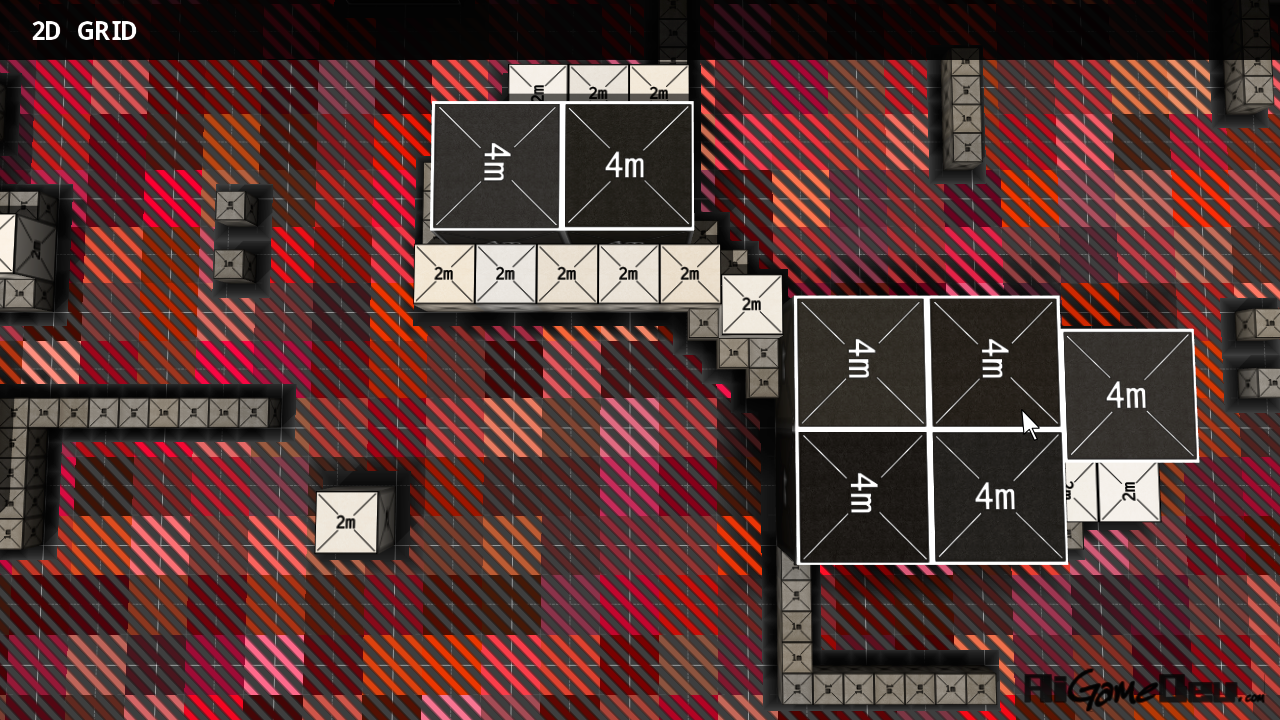
\includegraphics[width=0.8\linewidth]{Images/screenshot001_2dGrid}
		\caption[Fine Grid influence map]{Fine Grid \ac{IM}. The \ac{IM} of this thesis was also built in the same style. Thus the cells are small enough not to protrude over walls and objects. This is good for maps with few open spaces and narrow passages. \citep{gameDevInfluenceMap} \citep{imPathfinding}}
		\label{fig:screenshot0012dgrid}
	\end{figure}
	\begin{figure}[h!]
		\centering
		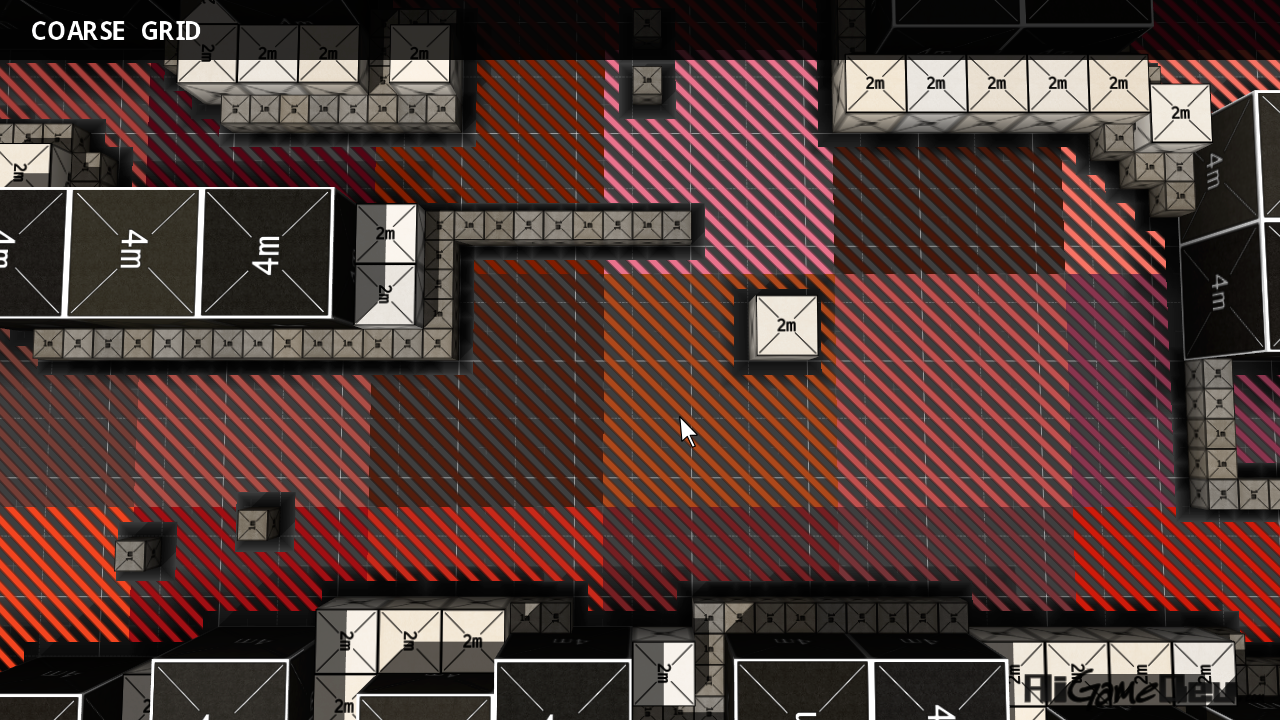
\includegraphics[width=0.8\linewidth]{Images/screenshot001_2dGrid2}
		\caption[Coarse grid influence map.]{Coarse grid \ac{IM}. With this map, large cells are placed on the map without taking into account whether the cell goes over the wall or not. This is good if you have open areas and few narrow passages. \citep{gameDevInfluenceMap} \citep{imPathfinding}}
		\label{fig:screenshot0012dgrid2}
	\end{figure}
	
	\newpage
	\subsubsection{Area Graph}
	
	\begin{figure}[h!]
		\centering
		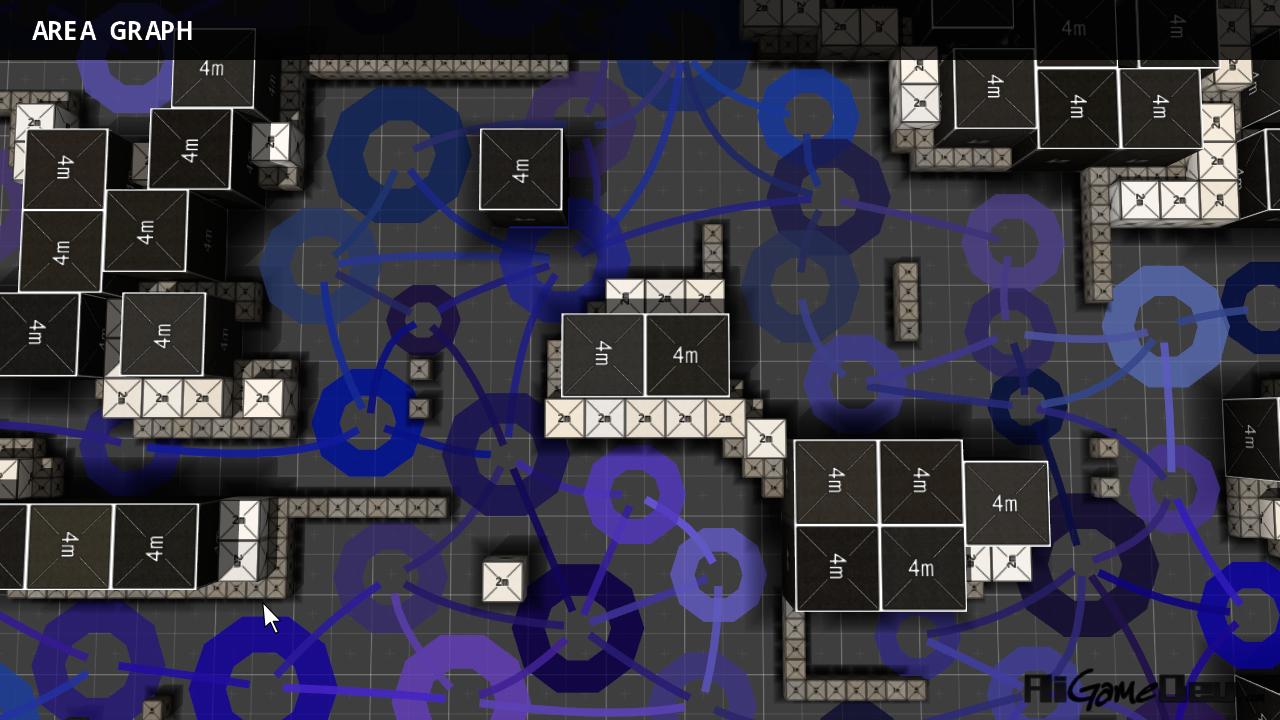
\includegraphics[width=0.8\linewidth]{Images/screenshot001_aregraph1}
		\caption[Area graph influence map.]{Area graph influence map. \citep{gameDevInfluenceMap} \citep{imPathfinding}}
		\label{fig:screenshot001aregraph1}
	\end{figure}
	
	\begin{figure}[h!]
		\centering
		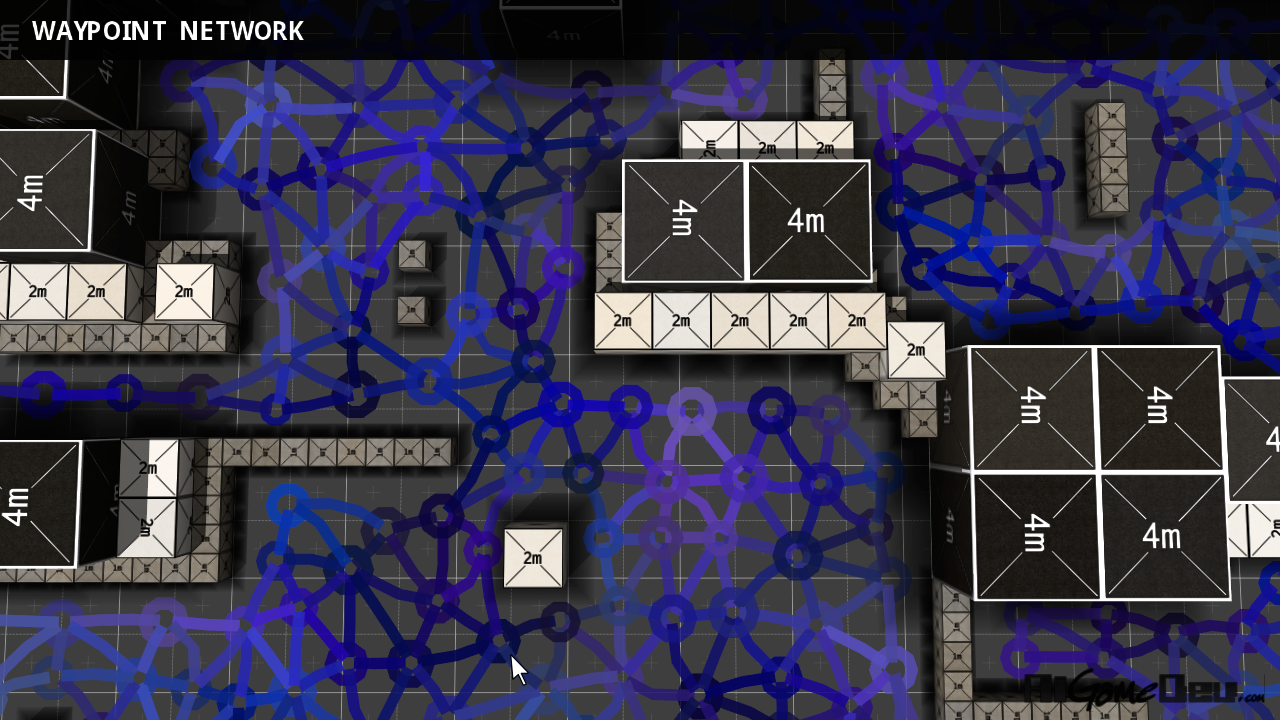
\includegraphics[width=0.8\linewidth]{Images/screenshot001_aregraph2}
		\caption[Waypoint network influence map.]{Waypoint network influence map. \citep{gameDevInfluenceMap} \citep{imPathfinding}}
		\label{fig:screenshot001aregraph2}
	\end{figure}
	
	\newpage
	\subsubsection{Properties}
	After setting the values of each agent in the IM, a blur algorithm is applied as explained in the chapter \ref{ssec:num1}. The choice of which blur method is best suited for each game depends heavily on the game designer. For example, depending on whether there are many walls on the level or more open vials, it can be decided whether to use one of the distance-based blur algorithms described in Chapter \ref{ssec:num2} or a blur algorithm from Chapter \ref{ssec:num1}. The important thing is to only apply this to cells that are accessible. Thus, the influence must propargize around walls and no distorted image is transmitted. The value from the blur algorithm is then multiplied by the decay to implement a decay of the influence on the range. 
	
	\begin{equation}
		I_{xy} = b_{xy} * D
	\end{equation}
	
	$I_{xy}$ is the influence at the point $x$ and $y$ in the grid. This is equal to the blurred value $b_{xy}$ at the point $x$ and $y$ from the algorithm multiplied by the decay value $D$.
	
	
	\begin{description}
		\item[$\bullet$ Momentum] With momentum the influence is linearly interpolated from the cell. In this way the memory of the IM is suggested.
		\begin{equation}
			I_{xy} = I_{xy} + ((I_{h} - I_{xy}) * m) 
		\end{equation}
		$I_{h}$ stands for the highest or lowest influence value that exists on the IM. If $I_{xy}$ is greater than or equal to $0$, the highest value is taken and if $I_{xy}$ is less than $0$, the lowest value is taken. $m$ is the value for the momentum. 
		
		\item[$\bullet$ Decay] Decay is for the decay of the influence value within an \ac{IM} so a kind of fading memory is built up and the influence continues to decrease depending on how far it is from its point of origin.
		\item[$\bullet$ Update Frequency] This parameter describes how often the influence is updated. 
		\end {description}
		
		\section{Blur } \label{ssec:num1}
		For the calculation of the influence on maps with narrow corridors and small areas a blur algorithm is used \citep{gameDevInfluenceMap}. \newline This suggests that the algorithm is not affected by obstacles. Thus the influence flows around the corners. In this work, a boxblur algorithm was applied. But it would work just as well with a Gaussian blur. This is open to the individual preferences of how the influence should spread. For this work, the boxblur algorithm was chosen because it provides a more uniform distribution in all directions of influence. 
		
		\begin{table}[H]
			\centering
			\begin{tabular}{|c|c|c|c|c|}
				\hline
				0.000 & 0.000 & 0.000 & 0.000 & 0.000\\
				\hline
				0.000 & \textbf{1.000} & 0.000 & 0.000 & 0.000\\
				\hline
				0.000 & 0.000 & 0.000 & 0.000 & 0.000\\
				\hline
				0.000 & 0.000 & 0.000 & 0.000 & 0.000\\
				\hline
				0.000 & 0.000 & \textbf{-1.000} & 0.000 & 0.000\\
				\hline
				
			\end{tabular}
			\caption{Boxblur influence example grid - Iteration 0. The inflow of two units was injected into a completely new \ac{IM}. The cell with the value $1.000$ is from the own team and the cell with the value $-1.000$ from the opposing team. }
			\label{tab:Boxblur grid Iteration 0}
		\end{table}
		
		The Box Blur is a spatial domain linear filter. It takes a pixel (or in our case a cell) from the grid and takes itself and its surrounding pixels and calculates the average as the new value. A 3 by 3 box blur (radius 1) can also be described as a matrix:
		
		\begin{equation}
			K = \frac{1}{9}\begin{bmatrix} 1 & 1 & 1\\ 1 & 1 & 1\\ 1 & 1 & 1 \end{bmatrix}
		\end{equation}
	
		$K$ is the average value of pixel and its surrounding values.\citep{boxblur}
		
		\begin{table}[H]
			\centering
			\begin{tabular}{|c|c|c|c|c|}
				\hline
				0.250 & 0.200 & 0.200 & 0.030 & 0.008\\
				\hline
				0.240 & \textbf{1.000} & 0.160 & 0.006 & 0.007\\
				\hline
				0.210 & 0.180 & 0.150 & 0.040 & 0.002\\
				\hline
				0.060 & -0.040 & -0.070 & -0.100 & -0.010\\
				\hline
				0.005 & -0.170 & \textbf{-1.000} & -0.200 & -0.078\\
				\hline
				
			\end{tabular}
			\caption{Boxblur influence example grid - Iteration 1. After the first iteration, from top left to bottom right, the cell was placed the 3 by 3 matrix. So that the center of the matrix lies on the cell and then calculated the mean value.}
			\label{tab:Boxblur grid Iteration 1}
		\end{table}
		
		\begin{table}[H]
			\centering
			\begin{tabular}{|c|c|c|c|c|}
				\hline
				0.420 & 0.370 & 0.290 & 0.080 & 0.025\\
				\hline
				0.400 & \textbf{1.000} & 0.250 & 0.009 & 0.027\\
				\hline
				0.300 & 0.250 & 0.140 & 0.030 & -0.007\\
				\hline
				0.068 & -0.057 & -0.130 & -0.15 & -0.069\\
				\hline
				-0.039 & -0.221 & \textbf{-1.000} & -0.271 & -0.142\\
				\hline
				
			\end{tabular}
			\caption{Boxblur influence example grid - Iteration 2}
			\label{tab:Boxblur grid Iteration 2}
		\end{table}
		
		Through this box blur, the influence is gradually expanded with $1.000$ and $-1.000$ and then stagnates after a certain iteration. The Celle with $1.000$ means that there is an allied unit that places its influence there and $-1.000$ means that there is an enemy unit.
		
		\section{Waypoints} \label{waypoint}
		Waypoints are positions distributed around the game world. With waypoints, the \ac{AI} can use this for its pathfinder in order to progress in the game world. Tactical waypoints require more data describing these points in order to make a correct decision about which waypoint to use \citep{AIforGamesTactical}.
		
		\chapter{Experimental setup}
		The expirement consists of a map on which two teams compete against each other. This will be similar to the game mode "Conquest" from Battlefield 1 \citep{battlefield1modes}. In Conquest, there are a certain number of places that a team tries to capture. At the beginning, each place is still uncaptured. When a team has taken a place, it always gets points added to their points account at certain time intervals. The team that has reached a certain number of points first after a certain time has won. 
		One side will consist of a squad of five agents, the other side of five squads of one agent each. A squad always knows where its agents are and whether a unit sees a friendly or enemy agent and can thus build up an \ac{IM}.
		When a team has won, information about the match is saved for later evaluation and the next match starts. This allows you to run this several thousand times so that the result is not falsified.
		
		\section{Game mode adjustments}
		Since in the game mode Conquest of Battlefield \citep{battlefield1modes} the current state of the capturable locations is always queried with a certain tick rate, this can lead to inaccurate values. Therefore the time a place is in possession of a team is counted to avoid the sampling problem.
		
		\section{Assumption} \label{assumption}
		The side with the squad and its five agents has a slightly higher win rate than the side with the 5 squads with one agent each. This is because it has more information to decide, for example, which of the points to attack first or which point may have no enemy units. 
		
		\section{Rules of the game}
		The goal of a match is to have captured capturable locations for the longest time. There are 3 capturable locations distributed for the agents. A location can be captured if there is no agent from the opposing team with an own agent at the location. In this case, the location's affiliation changes immediately. After the location is captured, the time is accumulated on the team's points account. The match ends after a total duration of 300 seconds. 
		During the match, the agents shoot at the opposing team then. Each agent has 100 health points and each shot that hits takes away 50 health points. If an agent dies, it will be instantiated again after 5 seconds. On a random location on the map that does not count as a capturable point but more about that in chapter \ref{ssec:rf}. 
		
		\subsection{Playing field construction}
		Two different types of maps are used. An open map where an agent can more easily discover own team members or enemy units and a closed map with many corridors to not promote the unknown as explained in chapter \ref{ssec:dwu}. The unknown is the \ac{FOW} that the agent cannot see on the map. 
		
		\subsubsection{Open map structure}
			\begin{figure}[h!]
			\centering
			\includegraphics[width=1\linewidth]{"Images/open map"}
			\caption[Open map structure]{An open map with three capturable points marked with a cyan rectangle.}
			\label{fig:open-map}
			\end{figure}
		
		\clearpage
		\subsubsection{Closed map Structure}
		\begin{figure}[h!]
			\centering
			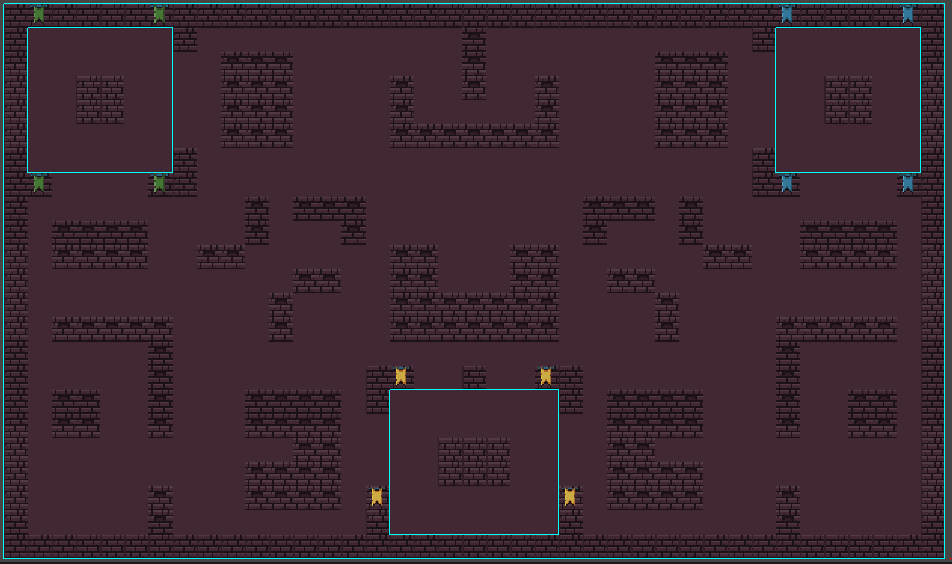
\includegraphics[width=1\linewidth]{Images/closemap}
			\caption[Close map structure]{A closed map with three capturable points marked with a cyan rectangle. Here are many angles and small corridors distributed on the map and it was careful not to have too many open spaces so that the influence must propagate more around the corners and that the agents are not very line of sight to own team members or opponents.}
			\label{fig:close-map}
		\end{figure}
		
		\subsection{Randomness factor} \label{ssec:rf}
		So that not every match runs the same, a random factor had to be added. Therefore the instantiation was chosen where an agent is placed when he died or when the match started. An agent then gets a random ball selected that is not in a capturable location. The randomization is done by the Unity3D engine random range function \citep{technologiesUnityRandomRange}. If you always play a round with the same spawn locations you will always get a deterministic result and the agents will make the same decisions.
		
		\clearpage
		\chapter{Results}
		The shared team means that a squad of 5 agents share an \ac{IM}. For the Unshared Team, it is 5 squads with one agent each. So each squad has its own \ac{IM} and does not know what the \ac{IM} of the other squad looks like from the team. 
		\section{Open map}
		\subsection{Shared vs Unshared}
		\begin{figure}[h!]
			\centering
			\includegraphics[width=0.9\linewidth]{"Images/100 Games Shared vs Unshared Open Map"}
			\caption[Shared vs Unshared - Open Map]{Shared vs Unshared - Open Map}
			\label{fig:100-games-shared-vs-unshared-open-map}
		\end{figure}
	In the run of Shared vs Unshared on the open map as seen here in Figure \ref{fig:open-map}, the Shared team won $53.0\%$ of $100$ runs. The team with the Unshared \ac{IM} won $47.0\%$.
		
		\clearpage
		\subsection{Unshared vs Shared}
		\begin{figure}[h!]
			\centering
			\includegraphics[width=0.9\linewidth]{"Images/100 Games Unshared vs Shared Open Map"}
			\caption[Unshared vs Shared - Open Map]{Unshared vs Shared - Open Map}
			\label{fig:100-games-unshared-vs-shared-open-map}
		\end{figure}
		In the run of Unshared vs Shared on the open map as seen here in Figure \ref{fig:open-map}, the Shared team won $36.0\%$ of $100$ runs. The team with the Unshared \ac{IM} won $64.0\%$. Shared and the Unshared team switched sides to see if it made a difference. 
		
		\clearpage
		\subsection{Shared vs Shared}
		\begin{figure}[h!]
			\centering
			\includegraphics[width=0.9\linewidth]{"Images/100 Games Shared vs Shared Open Map"}
			\caption[Shared vs Shared - Open Map]{Shared vs Shared - Open Map}
			\label{fig:100-games-shared-vs-shared-open-map}
		\end{figure}
		In the run of Shared vs Shared on the open map as seen here in Figure \ref{fig:open-map}, the blue Shared team won $57.0\%$ of $100$ runs. The orange team with the Shared \ac{IM} won $43.0\%$.
		
		\clearpage
		\subsection{Unshared vs Unshared}
		\begin{figure}[h!]
			\centering
			\includegraphics[width=0.9\linewidth]{"Images/100 Games Unshared vs Unshared Open Map"}
			\caption[Unshared vs Unshared - Open Map]{Unshared vs Unshared - Open Map}
			\label{fig:100-games-unshared-vs-unshared-open-map}
		\end{figure}
	In the run of Unshared vs Unshared on the open map as seen here in Figure \ref{fig:open-map}, the blue Unshared team won $60.0\%$ of $100$ runs. The orange team with the Unshared \ac{IM} won $40.0\%$.
		
		\clearpage
		\section{Closed map}
		\subsection{Shared vs Unshared}
		\begin{figure}[h!]
			\centering
			\includegraphics[width=0.9\linewidth]{"Images/100 Games Shared vs Unshared Close Map"}
			\caption[Shared vs Unshared - Closed Map]{Shared vs Unshared - Closed Map}
			\label{fig:100-games-shared-vs-unshared-close-map}
		\end{figure}
		In the run of Shared vs Unshared on the closed map as seen here in Figure \ref{fig:close-map}, the Shared team won $57.0\%$ of $100$ runs. The team with the Unshared \ac{IM} won $43.0\%$.
		
		\clearpage
		\subsection{Unshared vs Shared}
		\begin{figure}[h!]
			\centering
			\includegraphics[width=0.9\linewidth]{"Images/100 Games Unshared vs Shared Close Map"}
			\caption[Unshared vs Shared - Closed Map]{Unshared vs Shared - Closed Map}
			\label{fig:100-games-unshared-vs-shared-close-map}
		\end{figure}
	In the run of Unshared vs Shared on the closed map as seen here in Figure \ref{fig:close-map}, the Shared team won $73.0\%$ of $100$ runs. The team with the Unshared \ac{IM} won $27.0\%$.
		
		\clearpage
		\subsection{Shared vs Shared}
		\begin{figure}[h!]
			\centering
			\includegraphics[width=0.9\linewidth]{"Images/100 Games Shared vs Shared Close Map"}
			\caption[Shared vs Shared - Closed Map]{Shared vs Shared - Closed Map}
			\label{fig:100-games-shared-vs-shared-close-map}
		\end{figure}
		In the run of Shared vs Shared on the closed map as seen here in Figure \ref{fig:close-map}, the blue Shared team won $52.0\%$ of $100$ runs. The orange team with the Shared \ac{IM} won $48.0\%$.
		
		\clearpage\clearpage
		\subsection{Unshared vs Unshared}
		\begin{figure}[h!]
			\centering
			\includegraphics[width=0.9\linewidth]{"Images/100 Games Unshared vs Unshared Close Map"}
			\caption[Unshared vs Unshared - Closed Map]{Unshared vs Unshared - Closed Map}
			\label{fig:100-games-unshared-vs-unshared-close-map}
		\end{figure}
			In the run of Unshared vs Unshared on the closed map as seen here in Figure \ref{fig:close-map}, the blue Unshared team won $94.0\%$ of $100$ runs. The orange team with the Unshared \ac{IM} won $6.0\%$.
		
		
		\chapter{Discussion}
		As in Chapter \ref{assumption}, the assumption was that the team with the \ac{SK} from the \ac{IM} has a higher win rate than the team in which each agent has its own \ac{IM}. \newline
		What is immediately noticeable is that team 1 always wins in the 8 times 100 iterations, regardless of whether it is equipped with \ac{SK} or unshared knowledge. This can come from the fact that team 1 is the first in the calculation of the \ac{IM} from the sequential flow in the code. This could be one of the possibilities, but to confirm this would require running several 100 iteration packages of the respective team setup.
		
		\chapter{Conclusion}
		
		
		\newpage
		\chapter{Lists}
		\section*{List of Acronyms}
		\begin{acronym}[FOW]
			\acro{IM}{influence map}
			\acro{FOW}{fog-of-war}
			\acro{AI}{artificial intelligence}
			\acro{GDC}{game developers conference}
			\acro{SK}{shared knowledge}
			\acro{RTS}{Real Time Strategy}
		\end{acronym}
		
		\listoffigures
		\listoftables
		
		
		\bibliography{references}
	\end{document}
